\documentclass[titlepage]{article}
% \usepackage[margin=2.5cm]{geometry}
\usepackage[margin=2.5cm, headheight=0pt, headsep=1cm]{geometry}
\usepackage{enumerate, fancyhdr, graphicx, amsmath, nth}
\usepackage[binary-units=true]{siunitx}

\title{Hurricane Evacuation Strategies for the State of Mississippi}
\author{Paul Chesnais (pmc85), Antoine Pourchet (app63), and Ryan Vogan (rcv39)\\2015 Cornell Mathematical Contest in Modeling}
\date{November 16, 2015}

\pagestyle{fancy}
\fancyhead{}
\lhead{Chesnais, Pourchet, Vogan}
\chead{Hurricane Evacuation Strategies}
\rhead{November 16, 2015}
\fancyfoot{}
\rfoot{\thepage}
\renewcommand{\headrulewidth}{0.5pt}
\renewcommand{\footrulewidth}{0.5pt}

\usepackage{listings, color, times, textcomp, float, hyperref, setspace, subcaption}
\definecolor{Code}{rgb}{0,0,0}
\definecolor{Decorators}{rgb}{0.5,0.5,0.5}
\definecolor{Numbers}{rgb}{0.5,0,0}
\definecolor{MatchingBrackets}{rgb}{0.25,0.5,0.5}
\definecolor{Keywords}{rgb}{0,0,1}
\definecolor{self}{rgb}{0,0,0}
\definecolor{Strings}{rgb}{0,0.63,0}
\definecolor{Comments}{rgb}{0,0.63,1}
\definecolor{Backquotes}{rgb}{0,0,0}
\definecolor{Classname}{rgb}{0,0,0}
\definecolor{FunctionName}{rgb}{0,0,0}
\definecolor{Operators}{rgb}{0,0,0}
\definecolor{Background}{rgb}{0.98,0.98,0.98}
\definecolor{mygreen}{RGB}{28,172,0}
\definecolor{mylilas}{RGB}{170,55,241}

\lstdefinestyle{Python}{
  backgroundcolor=\color{Background},basicstyle=\ttfamily\small\setstretch{1},breaklines=true,
  commentstyle=\color{Comments}\slshape,emph={self},emphstyle={\color{self}\slshape},frame=l,framexbottommargin=2em,
  framextopmargin=2em,keywordstyle={[2]\color{Decorators}\slshape},keywordstyle={\color{Keywords}\bfseries},
  language=Python,morecomment=[s][\color{Strings}]{"""}{"""},morecomment=[s][\color{Strings}]{'''}{'''},
  morekeywords={[2]@invariant},morekeywords={import,from,class,def,for,while,if,is,in,elif,else,not,and,or,print,break,
  continue,return,True,False,None,access,as,del,except,exec,finally,global,import,lambda,pass,print,raise,try,assert},
  numbers=left,numbersep=1em,numberstyle=\footnotesize,showspaces=false,showstringspaces=false,showtabs=false,
  stringstyle=\color{Strings},tabsize=4,xleftmargin=1em,
}

\lstdefinestyle{Matlab}{
  backgroundcolor=\color{Background},basicstyle=\ttfamily\small\setstretch{1},breaklines=true,
  commentstyle=\color{mygreen},emph=[1]{for,end,break},emphstyle=[1]\color{red},frame=l,identifierstyle=\color{black},
  keywordstyle=[2]{\color{black}},keywordstyle=\color{blue},language=Matlab,literate={~} {\texttildelow}{1},
  morekeywords=[2]{1},morekeywords={matlab2tikz},numbers=left,numbersep=9pt,numberstyle={\tiny \color{black}},
  showstringspaces=false,stringstyle=\color{mylilas},
}

\begin{document}
\maketitle
\thispagestyle{empty}

\section{Executive Summary}
\label{sec:summary}

\section{Introduction}
\label{sec:introduction}
  The Mississippi Emergency Management Administration (MSEMA) has hired our team to design evacuation routes for at-risk counties in the coastal regions of southern Mississippi. Given that this coastal area is a strong commercial center, the governmental authorities want to minimize the number of unnecessary evacuations. Under this requirement, it is more advantageous to withhold ordering an evacuation for as long as possible. The reasons for this are two-fold. First, this ensures that local businesses can remain open for as long as possible. Second, this ensures that the forecasting reports at the time of the evacuation order are as accurate as possible. Therefore, our models seek to recommend an optimal evacuation plan as well as the latest possible time at which it is safe to enact this plan.

\section{Model Assumptions}
\label{sec:assumptions}
  The MSEMA specified that our plan should be enacted on a per-county basis. As you can see in the following figure, these counties are approximately equally sized:
  \begin{figure}[H]
  \centering
  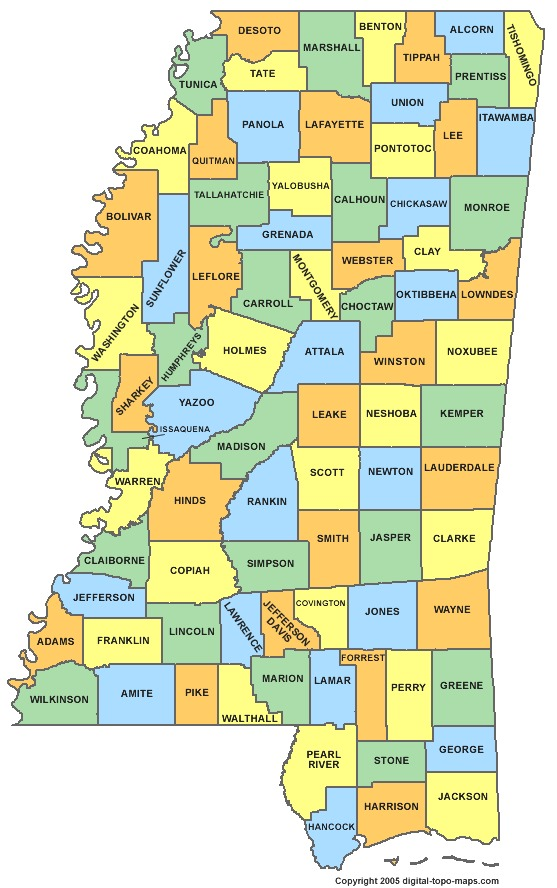
\includegraphics[width=.5\textwidth]{figures/county_map.jpg}
  \caption{A Map of Counties in the State of Mississippi \cite{county_map}}
  \end{figure}
  As a result of this, we assume that each county can be modeled as a single node in an undirected graph. Then an edge from node $i$ to node $j$ represents that a refugee can directly reach county $j$ from county $i$. Therefore, we constructed a network of Mississippi counties by connecting each county's node to the nodes of all bordering counties. This produced the following graph:
  \begin{figure}[H]
  \centering
  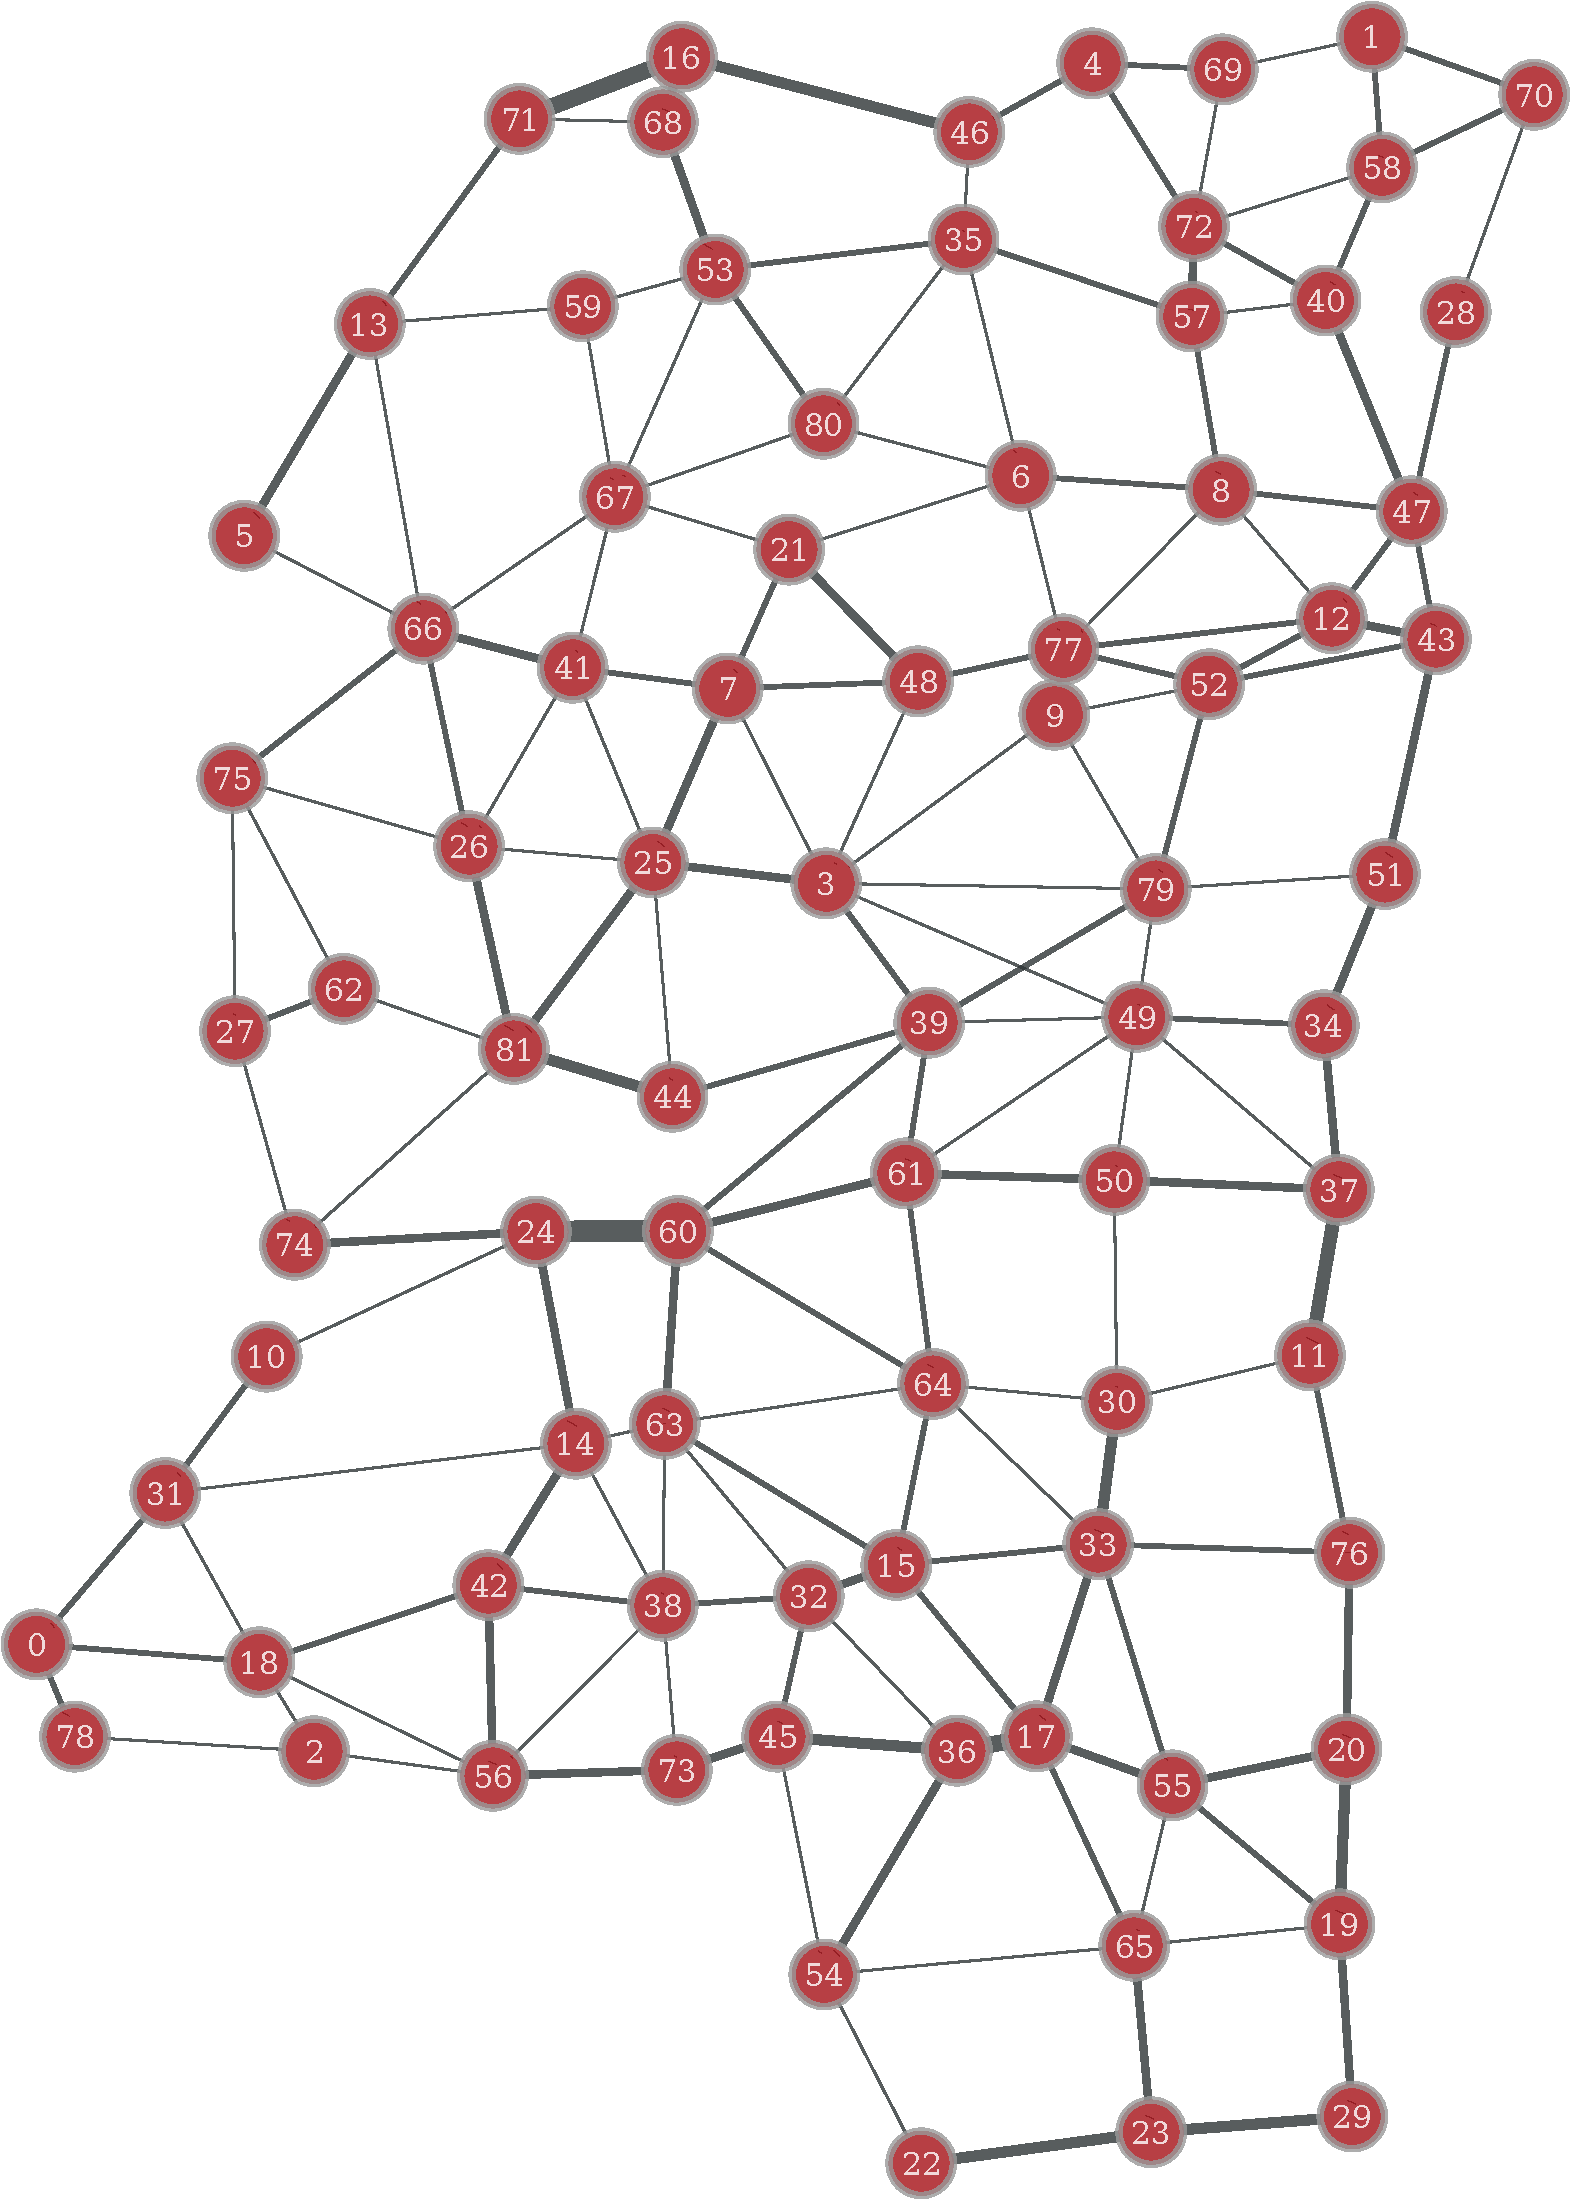
\includegraphics[width=.5\textwidth]{figures/full_undirected-crop.pdf}
  \caption{Undirected Graph Representing Mississippi Counties}
  \end{figure}
  Because Mississippi has varying highway structure, it would be inappropriate to assume uniform travel rates between county pairs. In order to capture this homogeneity in the network model, we decided to assign a weight to each edge. A single edge weight then represents a carrying capacity for the amount of travel possible between two counties. As a real world analogy, we assumed that this would correspond to the number of highway lanes traveling from one county to another. Therefore, we were able to assign edge weights across this graph by using the following highway map:
  \begin{figure}[H]
  \centering
  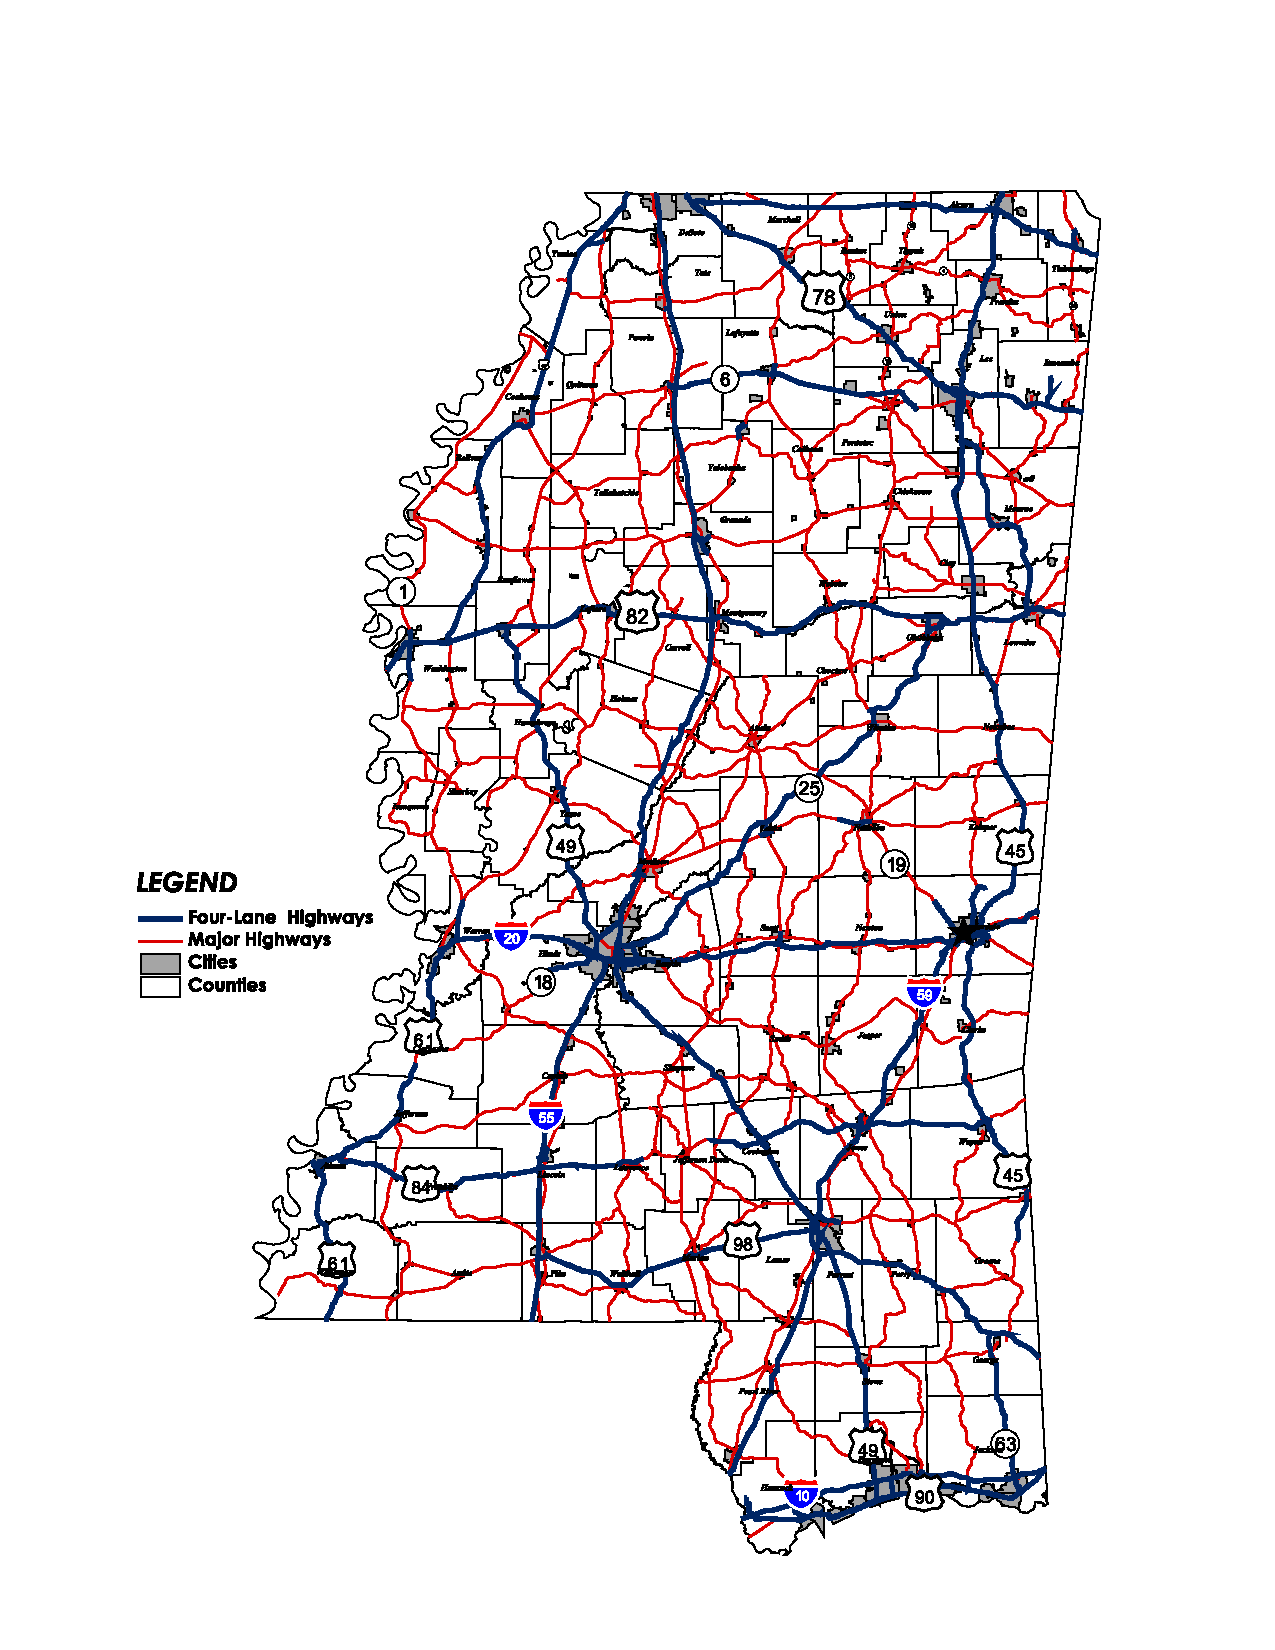
\includegraphics[width=.75\textwidth]{ms_highways.pdf}
  \caption{Map of Major Highways in the State of Mississippi \cite{ms_highways}}
  \end{figure}



\section{Statical Analysis of Historical Hurricane Data}
\label{sec:hurricanes}


\section{Markov Process Analysis of Strictly Northern Evacuations}
\label{sec:markov}
  \subsection{Model Description}
  \subsection{Parameter Values and Justification}
  \subsection{Results}
  \subsection{Strengths and Weaknesses}

\section{Maximum Flow Analysis of Strictly Northern Evacuations}
\label{sec:maxflow}
  \subsection{Model Description}
  \subsection{Parameter Values and Justification}
  \subsection{Results}
  \subsection{Strengths and Weaknesses}

\section{Stochastic Model of Landfall-Avodiant Evacuations}
\label{sec:stochastic}
  \subsection{Model Description}
    \par In this model, instead of giving citizens particular evacuation plan, we give them a simple rule: move directly away from the hurricane landfall if possible, else move North or North-West. Using the statewide broadcast system, the state of Mississippi can tell its citizens where the expected landfall will be, and which counties will be the most affected. In which case, individual citizens are instructed to leave the counties that will be flooded, and to do so as outlined above. This means less coordination from the state, and more options for each citizens. At the cost of not having designated areas, and therefore designated refuge areas for citizens, evacuation is faster because it involves less per-county organization.
  \subsection{Parameter Values and Justification}
    \par As opposed to the model described in \nameref{sec:maxflow}, we also allow citizens to leave the state of Mississippi. For example, Arkansas is less likely to be hit by the full force of hurricanes that move through Mississippi \cite{5news}, as such, it is a good place to take refuge while the storm passes. As such, we add ``unofficial'' nodes in the graph representation of Mississippi.
  \subsection{Results}

    \begin{figure}
      \center
      \begin{subfigure}[b]{0.5\textwidth}
        \center
        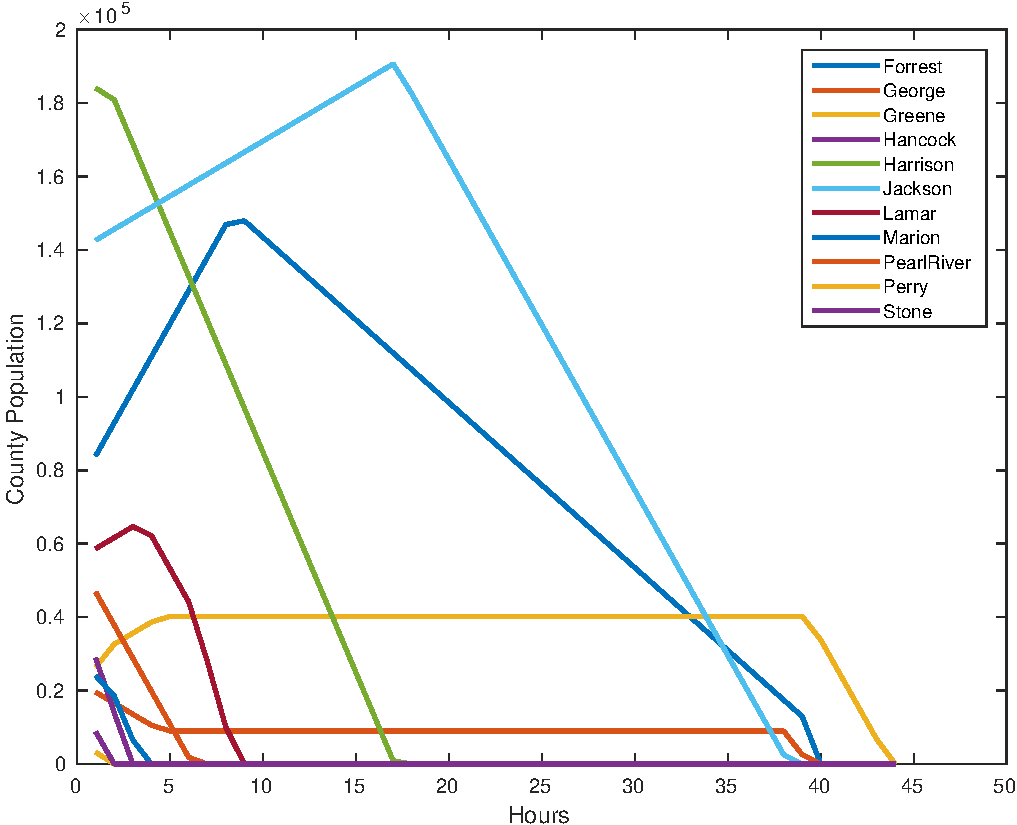
\includegraphics[width=\linewidth]{figures/pred_hancock-crop.pdf}
        \caption{Predicted Evacuation for Landfall in Hancock County}
      \end{subfigure}~
      \begin{subfigure}[b]{0.5\textwidth}
        \center
        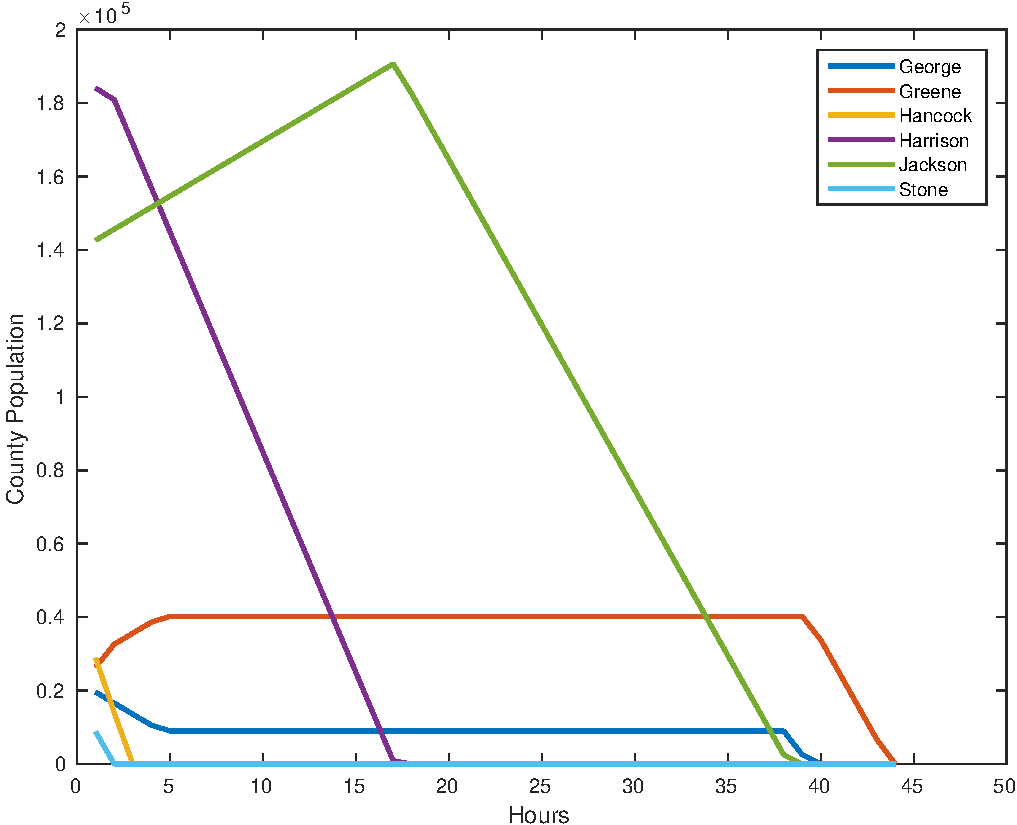
\includegraphics[width=\linewidth]{figures/pred_jackson-crop.pdf}
        \caption{Predicted Evacuation for Landfall in Jackson County}
      \end{subfigure}
      \caption{}
    \end{figure}
  \subsection{Strengths and Weaknesses}

\section{Conclusions}
\label{sec:conclusions}

\section{Future Work}
\label{sec:future}

\section{Individual Contributions}
\label{sec:contributions}
  \begin{thebibliography}{9}
    \bibitem{county_map}
      \url{http://www.madeinmississippi.us/wp-content/uploads/2015/02/mississippi-county-map.jpg}

    \bibitem{pmc}
      \url{http://www.ncbi.nlm.nih.gov/pmc/articles/PMC4060166/}

    \bibitem{5news}
      \url{http://5newsonline.com/2012/08/27/garretts-blog-hurricanes-in-arkansas/}

  \end{thebibliography}

\end{document}